\documentclass[../main.tex]{subfiles}
\begin{document}

\section{Setting up a Character Card}
When starting a new Character, find the Character's card. Fill in all the colored slots that have numbers or symbols in the Awakened, Buff, and Curse status columns. Place an Exhaustion token on the artwork of the card so that the face up side is the word white. 

\section{Health Bar}
At the top center of each Character card is a Health Bar for that Character. It lists the maximum amount of health that each unit belonging to that Character card has. Whenever a unit takes damage, place a marker in its health Bar for each damage taken. When ever a unit is healed by fish, loot, or other effects, remove a marker from its Health Bar for each health received. 

\begin{figure}[h]
    \centering
    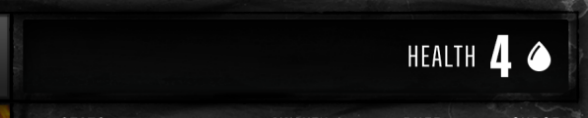
\includegraphics[width=1\linewidth]{chapters//Settingupacharactercard/TimeStrikeCharCardHealth.png}
\end{figure}

\textit{Note: Unit health cannot exceed the value labeled on its Health bar. }

\section{Character References}
Throughout the game there will be references to Characters and units. 

\subsection{Character}
When the term "Character" is used, this refers to all of the units associated with a single Character card. So, if a Character has two miniatures, they are both considered a single character. 

\begin{figure}[h]
    \centering
    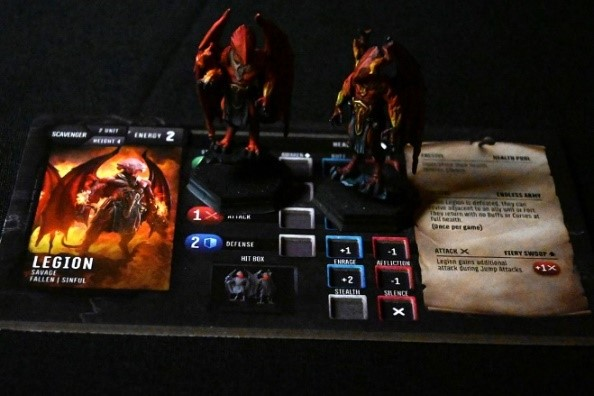
\includegraphics[width=1\linewidth]{chapters//Settingupacharactercard/TimeStrikeCharacterwithMini.jpg}
\end{figure}

\subsection{Unit}
When the term "unit" is used, this refers only to an individual miniature. Miniatures associated with Survivors, Monsters, Mobs, and the Sentience are all considered to be unit. 

\begin{figure}[h]
    \centering
    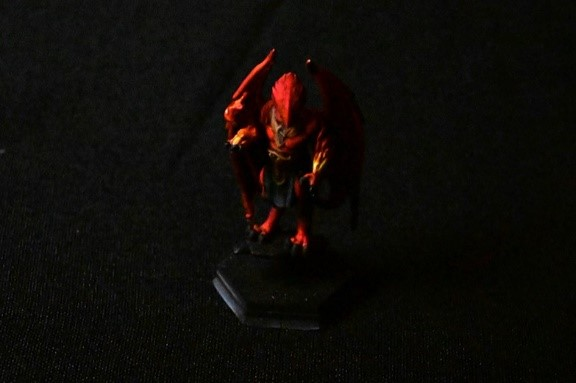
\includegraphics[width=0.75\linewidth]{chapters//Settingupacharactercard/TimeStrikeUnitMiniature.jpg}
\end{figure}

\subsection{Multi-unit Characters}
Certain Characters cards will have a unit count greater than 1. These are multi-unit Characters. When taking a turn with a multi-unit Character, each unit is activated individually and performs its own separate movement and actions, but they are all considered to belong to a single Character. Each unit also received damage individually, unless they have an ability stated otherwise. 

\begin{figure}[h]
    \centering
    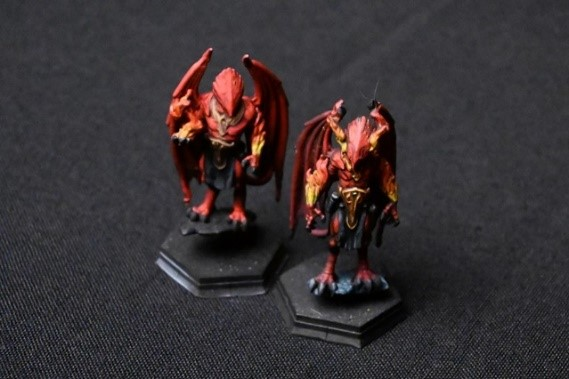
\includegraphics[width=0.75\linewidth]{chapters//Settingupacharactercard/TimeStrikeMultiunitMinis.jpg}
\end{figure}

\subsection{Multi-hex Units}
Some units are so large that they take up multiple hexes. These are referred to as multi-hex units. 
\begin{figure}[h]
    \centering
    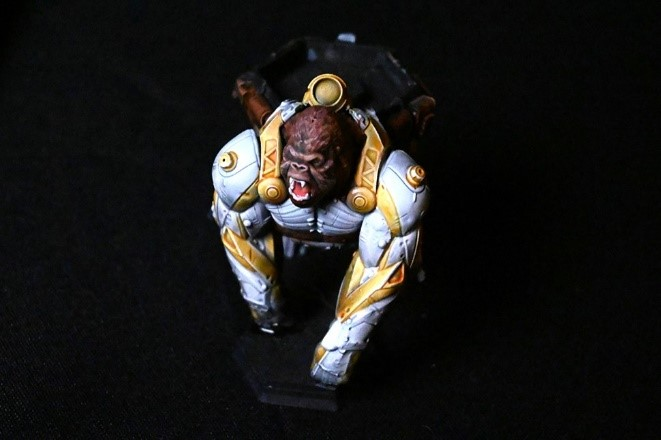
\includegraphics[width=0.75\linewidth]{chapters//Settingupacharactercard/TimeStrikeMultihexmini.jpeg}
\end{figure}

\subsection{Lost}
The lost refers to units on the board that are not controlled by players. They are instead controlled by the game. 


\subsection{Monster}
Monsters are types of Characters within the lost that start controlled by the Sentience and can be tamed and controlled by players. 

\subsection{Roles}
Roles associate Characters with specific mechanics. The list of roles includes Survivors, Brutes, and Beasts. 

\begin{itemize}
    \item \textbf{Survivors} are Characters that can be initially drafted onto each player's team. 
    \item \textbf{Beasts} are a type of Monster Character, controlled by the Sentience, that start on the board and can be summoned in. When tamed, they act as a multi-unit.
    \item \textbf{Brutes} are a type of Monster Character, controlled by the Sentience that will be summoned onto the board. When tamed, the Character mounts the Brute. 
\end{itemize}

\clearpage

\end{document}
